\section{Model2DRigid\-Car\-Smooth\-Trailer  Class Reference}
\label{classModel2DRigidCarSmoothTrailer}\index{Model2DRigidCarSmoothTrailer@{Model2DRigid\-Car\-Smooth\-Trailer}}
A rigid car-like robot with continuous steering angles and a trailer. The trailer models are taken from Murray and Sastry, Trans. Automatic Control, Vol 38, No 5, 1993, pp. 700-716. 


{\tt \#include $<$model2d.h$>$}

Inheritance diagram for Model2DRigid\-Car\-Smooth\-Trailer::\begin{figure}[H]
\begin{center}
\leavevmode
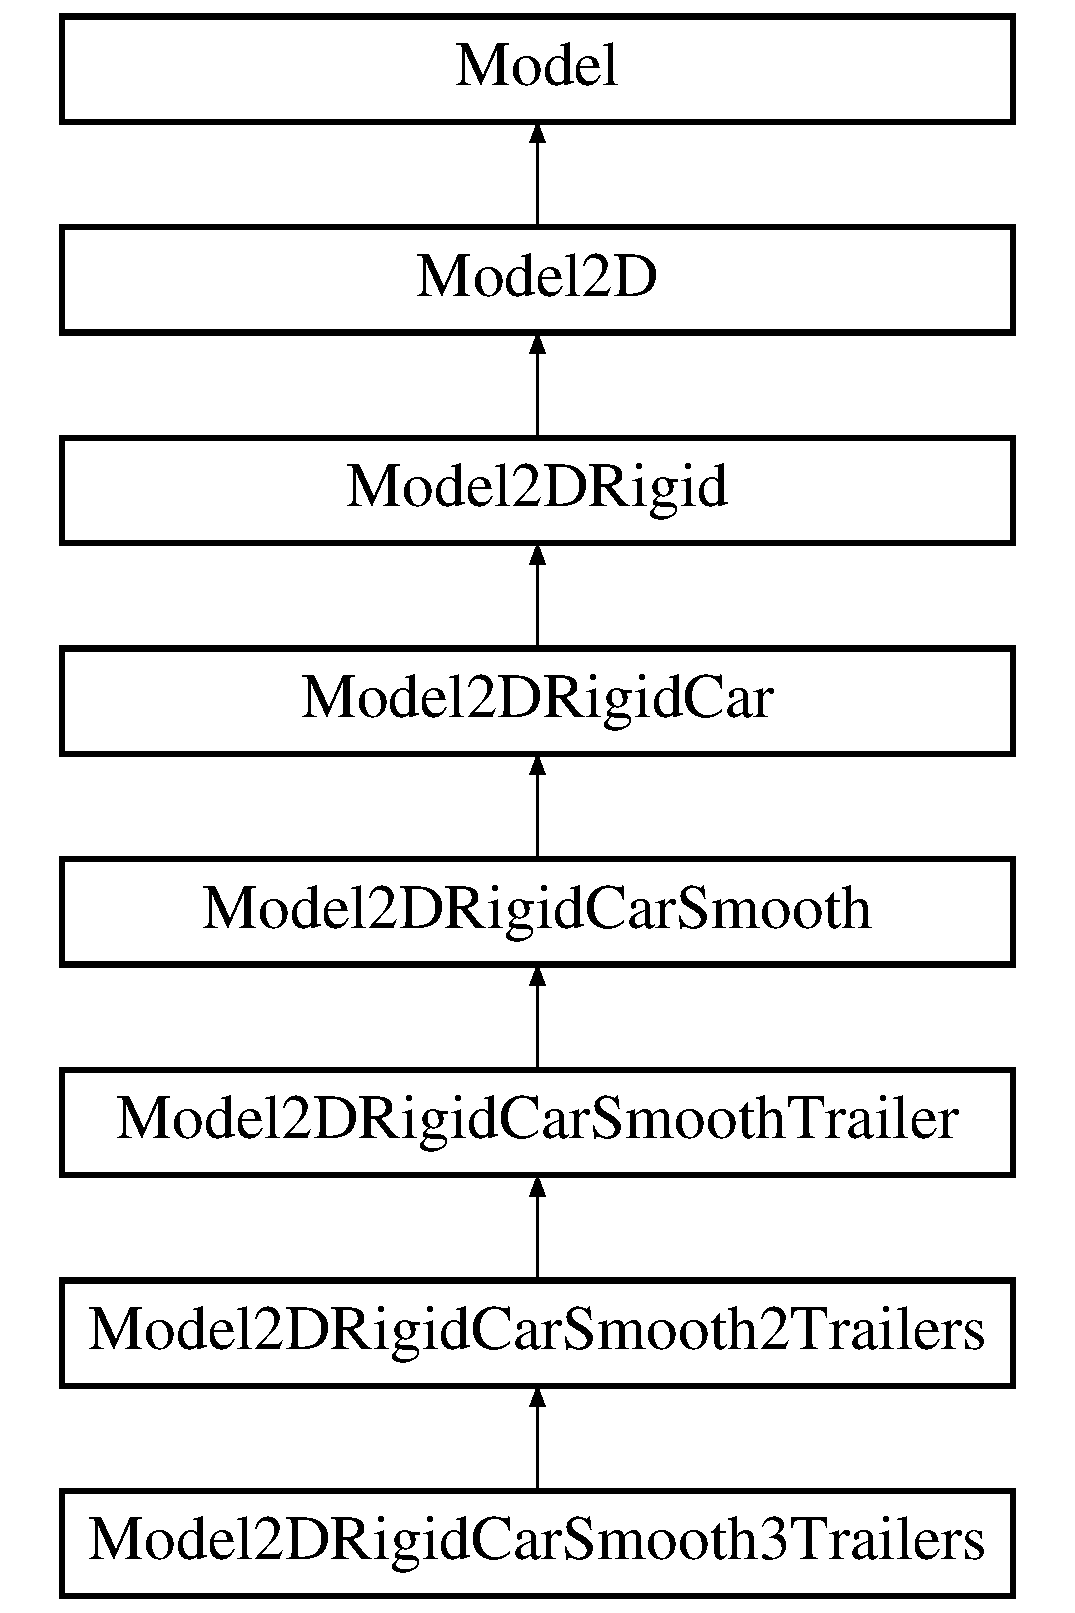
\includegraphics[height=8cm]{classModel2DRigidCarSmoothTrailer}
\end{center}
\end{figure}
\subsection*{Public Methods}
\begin{CompactItemize}
\item 
{\bf Model2DRigid\-Car\-Smooth\-Trailer} (string path)
\item 
virtual {\bf $\sim$Model2DRigid\-Car\-Smooth\-Trailer} ()
\item 
virtual {\bf MSLVector} {\bf State\-Transition\-Equation} (const {\bf MSLVector} \&{\bf x}, const {\bf MSLVector} \&u)
\begin{CompactList}\small\item\em The state transition equation, or equations of motion, xdot=f(x,u).\item\end{CompactList}\item 
virtual double {\bf Metric} (const {\bf MSLVector} \&x1, const {\bf MSLVector} \&x2)
\begin{CompactList}\small\item\em A distance metric, which is Euclidean in the base class.\item\end{CompactList}\item 
virtual {\bf MSLVector} {\bf State\-To\-Configuration} (const {\bf MSLVector} \&{\bf x})
\begin{CompactList}\small\item\em A method that converts a {\bf Model} {\rm (p.\,\pageref{classModel})} state in to a {\bf Geom} {\rm (p.\,\pageref{classGeom})} configuration.\item\end{CompactList}\item 
virtual bool {\bf Satisfied} (const {\bf MSLVector} \&{\bf x})
\begin{CompactList}\small\item\em Test whether global state-space constraints are satisfied.\item\end{CompactList}\end{CompactItemize}
\subsection*{Public Attributes}
\begin{CompactItemize}
\item 
double {\bf Hitch\-Length}
\item 
double {\bf Hitch\-Max\-Angle}
\end{CompactItemize}


\subsection{Detailed Description}
A rigid car-like robot with continuous steering angles and a trailer. The trailer models are taken from Murray and Sastry, Trans. Automatic Control, Vol 38, No 5, 1993, pp. 700-716.



\subsection{Constructor \& Destructor Documentation}
\index{Model2DRigidCarSmoothTrailer@{Model2DRigid\-Car\-Smooth\-Trailer}!Model2DRigidCarSmoothTrailer@{Model2DRigidCarSmoothTrailer}}
\index{Model2DRigidCarSmoothTrailer@{Model2DRigidCarSmoothTrailer}!Model2DRigidCarSmoothTrailer@{Model2DRigid\-Car\-Smooth\-Trailer}}
\subsubsection{\setlength{\rightskip}{0pt plus 5cm}Model2DRigid\-Car\-Smooth\-Trailer::Model2DRigid\-Car\-Smooth\-Trailer (string {\em path})}\label{classModel2DRigidCarSmoothTrailer_a0}


\index{Model2DRigidCarSmoothTrailer@{Model2DRigid\-Car\-Smooth\-Trailer}!~Model2DRigidCarSmoothTrailer@{$\sim$Model2DRigidCarSmoothTrailer}}
\index{~Model2DRigidCarSmoothTrailer@{$\sim$Model2DRigidCarSmoothTrailer}!Model2DRigidCarSmoothTrailer@{Model2DRigid\-Car\-Smooth\-Trailer}}
\subsubsection{\setlength{\rightskip}{0pt plus 5cm}virtual Model2DRigid\-Car\-Smooth\-Trailer::$\sim$Model2DRigid\-Car\-Smooth\-Trailer ()\hspace{0.3cm}{\tt  [inline, virtual]}}\label{classModel2DRigidCarSmoothTrailer_a1}




\subsection{Member Function Documentation}
\index{Model2DRigidCarSmoothTrailer@{Model2DRigid\-Car\-Smooth\-Trailer}!Metric@{Metric}}
\index{Metric@{Metric}!Model2DRigidCarSmoothTrailer@{Model2DRigid\-Car\-Smooth\-Trailer}}
\subsubsection{\setlength{\rightskip}{0pt plus 5cm}double Model2DRigid\-Car\-Smooth\-Trailer::Metric (const {\bf MSLVector} \& {\em x1}, const {\bf MSLVector} \& {\em x2})\hspace{0.3cm}{\tt  [virtual]}}\label{classModel2DRigidCarSmoothTrailer_a3}


A distance metric, which is Euclidean in the base class.



Reimplemented from {\bf Model2DRigid\-Car\-Smooth} {\rm (p.\,\pageref{classModel2DRigidCarSmooth_a3})}.

Reimplemented in {\bf Model2DRigid\-Car\-Smooth2Trailers} {\rm (p.\,\pageref{classModel2DRigidCarSmooth2Trailers_a3})}.\index{Model2DRigidCarSmoothTrailer@{Model2DRigid\-Car\-Smooth\-Trailer}!Satisfied@{Satisfied}}
\index{Satisfied@{Satisfied}!Model2DRigidCarSmoothTrailer@{Model2DRigid\-Car\-Smooth\-Trailer}}
\subsubsection{\setlength{\rightskip}{0pt plus 5cm}bool Model2DRigid\-Car\-Smooth\-Trailer::Satisfied (const {\bf MSLVector} \& {\em x})\hspace{0.3cm}{\tt  [virtual]}}\label{classModel2DRigidCarSmoothTrailer_a5}


Test whether global state-space constraints are satisfied.



Reimplemented from {\bf Model2DRigid\-Car\-Smooth} {\rm (p.\,\pageref{classModel2DRigidCarSmooth_a5})}.

Reimplemented in {\bf Model2DRigid\-Car\-Smooth2Trailers} {\rm (p.\,\pageref{classModel2DRigidCarSmooth2Trailers_a5})}.\index{Model2DRigidCarSmoothTrailer@{Model2DRigid\-Car\-Smooth\-Trailer}!StateToConfiguration@{StateToConfiguration}}
\index{StateToConfiguration@{StateToConfiguration}!Model2DRigidCarSmoothTrailer@{Model2DRigid\-Car\-Smooth\-Trailer}}
\subsubsection{\setlength{\rightskip}{0pt plus 5cm}{\bf MSLVector} Model2DRigid\-Car\-Smooth\-Trailer::State\-To\-Configuration (const {\bf MSLVector} \& {\em x})\hspace{0.3cm}{\tt  [virtual]}}\label{classModel2DRigidCarSmoothTrailer_a4}


A method that converts a {\bf Model} {\rm (p.\,\pageref{classModel})} state in to a {\bf Geom} {\rm (p.\,\pageref{classGeom})} configuration.



Reimplemented from {\bf Model2DRigid\-Car\-Smooth} {\rm (p.\,\pageref{classModel2DRigidCarSmooth_a4})}.

Reimplemented in {\bf Model2DRigid\-Car\-Smooth2Trailers} {\rm (p.\,\pageref{classModel2DRigidCarSmooth2Trailers_a4})}.\index{Model2DRigidCarSmoothTrailer@{Model2DRigid\-Car\-Smooth\-Trailer}!StateTransitionEquation@{StateTransitionEquation}}
\index{StateTransitionEquation@{StateTransitionEquation}!Model2DRigidCarSmoothTrailer@{Model2DRigid\-Car\-Smooth\-Trailer}}
\subsubsection{\setlength{\rightskip}{0pt plus 5cm}{\bf MSLVector} Model2DRigid\-Car\-Smooth\-Trailer::State\-Transition\-Equation (const {\bf MSLVector} \& {\em x}, const {\bf MSLVector} \& {\em u})\hspace{0.3cm}{\tt  [virtual]}}\label{classModel2DRigidCarSmoothTrailer_a2}


The state transition equation, or equations of motion, xdot=f(x,u).



Reimplemented from {\bf Model2DRigid\-Car\-Smooth} {\rm (p.\,\pageref{classModel2DRigidCarSmooth_a2})}.

Reimplemented in {\bf Model2DRigid\-Car\-Smooth2Trailers} {\rm (p.\,\pageref{classModel2DRigidCarSmooth2Trailers_a2})}.

\subsection{Member Data Documentation}
\index{Model2DRigidCarSmoothTrailer@{Model2DRigid\-Car\-Smooth\-Trailer}!HitchLength@{HitchLength}}
\index{HitchLength@{HitchLength}!Model2DRigidCarSmoothTrailer@{Model2DRigid\-Car\-Smooth\-Trailer}}
\subsubsection{\setlength{\rightskip}{0pt plus 5cm}double Model2DRigid\-Car\-Smooth\-Trailer::Hitch\-Length}\label{classModel2DRigidCarSmoothTrailer_m0}


\index{Model2DRigidCarSmoothTrailer@{Model2DRigid\-Car\-Smooth\-Trailer}!HitchMaxAngle@{HitchMaxAngle}}
\index{HitchMaxAngle@{HitchMaxAngle}!Model2DRigidCarSmoothTrailer@{Model2DRigid\-Car\-Smooth\-Trailer}}
\subsubsection{\setlength{\rightskip}{0pt plus 5cm}double Model2DRigid\-Car\-Smooth\-Trailer::Hitch\-Max\-Angle}\label{classModel2DRigidCarSmoothTrailer_m1}




The documentation for this class was generated from the following files:\begin{CompactItemize}
\item 
{\bf model2d.h}\item 
{\bf model2d.C}\end{CompactItemize}
